% Source: chain_rule_to_bptt.tex
\begin{notechapter}
% ---- chapter-local definitions ----
\forgetenv{keyinsight}\newtcolorbox{keyinsight}[1][]{
    colback=blue!5!white,
    colframe=blue!75!black,
    title=\textbf{Key Insight},
    #1
}
\forgetenv{warning}\newtcolorbox{warning}[1][]{
    colback=orange!5!white,
    colframe=orange!75!black,
    title=\textbf{Important Note},
    #1
}
\forgetcs\matrixSlice\newcommand{\matrixSlice}[1]{%
    $\begin{bNiceMatrix}
        a_{11}^{#1} & \Cdots & a_{1n}^{#1} \\
        \Vdots & \Ddots & \Vdots \\
        a_{m1}^{#1} & \Cdots & a_{mn}^{#1}
    \end{bNiceMatrix}$
}
% -----------------------------------
\chapter{From the Chain Rule to Backpropagation Through Time}\label{ch:chain-rule-to-bptt}
\chaptersubtitle{A complete mathematical journey from first principles to recurrent neural networks}

\begin{abstract}
This document provides a comprehensive pedagogical journey from the fundamental
multivariable chain rule to its sophisticated application in training recurrent
neural networks via Backpropagation Through Time (BPTT). We begin with a
rigorous derivation of the chain rule following Hubbard's linear approximation
approach, illustrate with concrete examples, and then systematically extend
these principles to the temporal unfolding of recurrent networks.

\textbf{Key features of this document:}
\begin{itemize}[leftmargin=*,itemsep=0pt]
    \item Complete mathematical derivations from first principles
    \item Detailed tensor calculus with 3D visualizations
    \item Element-wise to matrix-form progression for gradient computations
    \item Explicit worked examples with step-by-step calculations
    \item Beautiful diagrams showing RNN architecture and computational graphs
\end{itemize}

This treatment emphasizes both mathematical rigor and practical understanding,
building intuition through detailed explanations and visual aids.
\end{abstract}

\section{Introduction}
The chain rule is a fundamental tool in calculus that allows us to compute
derivatives of composed functions. In machine learning, and particularly in deep
learning, the chain rule is the mathematical backbone of the backpropagation
algorithm used to train neural networks. This document traces a complete
mathematical path from the multivariable chain rule to its application in
recurrent neural networks through Backpropagation Through Time (BPTT).

\subsection{Why This Document?}

Many treatments of BPTT either:
\begin{itemize}[leftmargin=*]
    \item Jump directly to matrix formulas without showing how they arise from first principles
    \item Skip the detailed tensor calculus that explains gradient computation
    \item Omit the connection between abstract derivatives and concrete implementations
\end{itemize}

This document aims to fill these gaps by providing:
\begin{enumerate}[leftmargin=*]
    \item \textbf{Rigorous foundations}: Starting from Hubbard's definition of differentiability as linear approximation
    \item \textbf{Complete derivations}: Every gradient formula derived from element-wise computations through tensor calculus to final matrix form
    \item \textbf{Visual understanding}: 3D tensor visualizations and computational graphs that build intuition
    \item \textbf{Worked examples}: Concrete calculations that verify abstract formulas
\end{enumerate}

\subsection{Document Roadmap}

\textbf{Section 2: Chain Rule Foundations}
\begin{itemize}[leftmargin=*,itemsep=0pt]
    \item Rigorous derivation from differentiability definition
    \item Jacobian matrix construction
    \item Chain rule theorem and proof
    \item Concrete worked examples
\end{itemize}

\textbf{Section 3: Backpropagation Through Time}
\begin{itemize}[leftmargin=*,itemsep=0pt]
    \item RNN architecture and notation
    \item Computational graph unfolding
    \item \textbf{Detailed tensor gradient computations} (the heart of this document)
    \item Parameter gradient formulas
    \item Complete BPTT algorithm
\end{itemize}

\begin{keyinsight}
The key pedagogical approach of this document is to show gradients at three
levels:
\begin{enumerate}
    \item \textbf{Element-wise}: How individual scalar derivatives combine
    \item \textbf{Tensor form}: How derivatives organize into higher-dimensional arrays
    \item \textbf{Matrix form}: How to implement these computations efficiently
\end{enumerate}
This progression builds deep understanding of what matrix operations actually
represent.
\end{keyinsight}

\section{Chain Rule}

\subsection{Context and Notation}

\textbf{Notation Convention for Derivatives:}
Throughout this document, we use the following consistent notational convention:
\begin{itemize}[leftmargin=*,itemsep=2pt]
    \item $\frac{\partial f}{\partial \mathbf{x}}$ denotes the \textbf{Jacobian matrix} (the derivative operator)
    \begin{itemize}
        \item If $f: \mathbb{R}^n \to \mathbb{R}$ (scalar function): Jacobian is a $1 \times n$ row vector
        \item If $\mathbf{f}: \mathbb{R}^n \to \mathbb{R}^m$ (vector function): Jacobian is an $m \times n$ matrix
        \item Entry $(i,j)$ is $\frac{\partial f_i}{\partial x_j}$
    \end{itemize}
    \item $\nabla_{\mathbf{x}} f$ denotes the \textbf{gradient} (only for scalar functions)
    \begin{itemize}
        \item This is an $n \times 1$ column vector
        \item Relationship: $\nabla_{\mathbf{x}} f = \left(\frac{\partial f}{\partial \mathbf{x}}\right)^\mathsf{T}$
    \end{itemize}
    \item The chain rule for scalar composition $f \circ \mathbf{g}$ gives:
    \[
    \frac{\partial (f \circ \mathbf{g})}{\partial \mathbf{x}} = \frac{\partial f}{\partial \mathbf{u}} \frac{\partial \mathbf{g}}{\partial \mathbf{x}}
    \quad \text{(Jacobian form: row × matrix)}
    \]
    In gradient form (transposing both sides):
    \[
    \nabla_{\mathbf{x}}(f \circ \mathbf{g}) = \left(\frac{\partial \mathbf{g}}{\partial \mathbf{x}}\right)^\mathsf{T} \nabla_{\mathbf{u}} f
    \quad \text{(column = matrix}^\mathsf{T} \text{ column)}
    \]
\end{itemize}

\begin{keyinsight}[title=Why This Convention?]
The notation $\frac{\partial}{\partial \mathbf{x}}$ \textbf{always represents 
the derivative/Jacobian matrix}, whether the function is scalar or 
vector-valued. This is the fundamental derivative operator. The gradient 
$\nabla$ is a special case (for scalar functions only) defined as the 
transpose of the Jacobian row vector.

This keeps the notation consistent with the chain rule: Jacobians multiply 
as matrices.
\end{keyinsight}

\begin{warning}[title=Machine Learning Convention vs Mathematical Rigor]
In machine learning literature, you will often see expressions like 
``$\frac{\partial L}{\partial \mathbf{W}}$'' referred to as the 
\textbf{gradient}, even though mathematically this is the \textbf{Jacobian}. 
This is because:
\begin{itemize}[itemsep=0pt]
    \item In ML, we primarily care about scalar loss functions
    \item The term ``gradient descent'' is universally used
    \item The distinction between Jacobian (row) and gradient (column) is 
    often glossed over
\end{itemize}

However, for mathematical rigor, we maintain the distinction in this document:
\begin{itemize}[itemsep=0pt]
    \item $\frac{\partial L}{\partial \mathbf{W}}$ is the 
    \textbf{Jacobian} (derivative)
    \item $\nabla_{\mathbf{W}} L = \left(\frac{\partial L}{\partial 
    \mathbf{W}}\right)^\mathsf{T}$ is the \textbf{gradient}
\end{itemize}

This precision is crucial for understanding the transpose operations in 
backpropagation formulas!
\end{warning}

\vspace{1em}

Consider a scalar-valued function of a vector:
\begin{equation*}
    y = f(\mathbf{u}) \in \mathbb{R} \text{ with } \mathbf{u} =
    \begin{bmatrix}
        u_1 \\ \vdots \\ u_m
    \end{bmatrix}
    \in \mathbb{R}^{m}
\end{equation*}
Suppose each $u_{i} = g_i(\mathbf{x})$ with $\mathbf{x} = 
\begin{bmatrix}
        x_1 \\ \vdots \\ x_n
    \end{bmatrix}
\in \mathbb{R}^{n}$.\\
So, each $g_i$ is a function from $\mathbb{R}^{n}$ to $\mathbb{R}$.\\
We can write this composition as:
\begin{align*}
    \mathbf{u} = g(\mathbf{x}) \in \mathbb{R}^m \text{ with } g&\colon \mathbb{R}^{n} \longrightarrow \, \mathbb{R}^{m} \\
    &\begin{bmatrix}
        x_1 \\ \vdots \\ x_n
    \end{bmatrix}
    \mapsto
    \begin{bmatrix}
        g_1(\mathbf{x}) \\ \vdots \\ g_m(\mathbf{x})
    \end{bmatrix}
\end{align*}
Thus, we have:
\begin{equation}\label{chain-rule-to-bptt:eq:fog}
    y = f(\mathbf{u}) = f(g(\mathbf{x})) = f\Bigg(
        \begin{bmatrix}
            g_1(\mathbf{x}) \\ \vdots \\ g_m(\mathbf{x})
        \end{bmatrix}
        \Bigg)
        \in \mathbb{R}
\end{equation}

\subsection{Rigorous Derivation of the Multivariable Chain Rule}

Following Hubbard's approach, we start with the fundamental idea of
differentiability as the existence of a \textit{good linear approximation}.

\subsubsection{From Differentiability to Partial Derivatives}

If $g$ is differentiable at $\mathbf{a}$, then by definition there exists a
linear transformation $[Dg(\mathbf{a})]$ such that:

\[
\lim_{\mathbf{h} \to \mathbf{0}} \frac{\|g(\mathbf{a} + \mathbf{h}) - g(\mathbf{a}) - [Dg(\mathbf{a})]\mathbf{h}\|}{\|\mathbf{h}\|} = 0.
\tag{D}
\]

Let us examine the consequence of (D) when $\mathbf{h}$ points along the $j$-th
coordinate axis. Take $\mathbf{h} = h\mathbf{e}_j$, where $\mathbf{e}_j$ is the
$j$-th standard basis vector and $h$ is a real number. Since $\|\mathbf{h}\| =
|h|$, condition (D) becomes:

\[
\lim_{h \to 0} \frac{\|\,g(\mathbf{a} + h\mathbf{e}_j) - g(\mathbf{a}) - h\,[Dg(\mathbf{a})]\mathbf{e}_j\,\|}{|h|} = 0.
\tag{CR.1}
\]

Define the auxiliary vector
\[
\mathbf{v}(h) \;:=\; \frac{g(\mathbf{a} + h\mathbf{e}_j) - g(\mathbf{a})}{h} \;-\; [Dg(\mathbf{a})]\mathbf{e}_j .
\]

A simple algebraic manipulation shows that
\[
\frac{g(\mathbf{a} + h\mathbf{e}_j) - g(\mathbf{a}) - h\,[Dg(\mathbf{a})]\mathbf{e}_j}{|h|}
= \mathbf{v}(h)\,\frac{h}{|h|}.
\]

Because $|h/|h|| = 1$, the norm of the right‑hand side equals
$\|\mathbf{v}(h)\|$. Equation (CR.1) therefore reads
\[
\lim_{h \to 0} \|\mathbf{v}(h)\| = 0.
\tag{CR.2}
\]

Now we use a basic fact about norms on $\mathbb{R}^m$: if a sequence (or a
function) of vectors converges to zero in norm, then each of its components
converges to zero. More precisely, for the Euclidean norm $\|\cdot\|$ one has
the inequality $|w_i| \le \|\mathbf{w}\|$ for every component $w_i$ of a vector
$\mathbf{w}$. Applying this to $\mathbf{v}(h)$ gives
\[
|\,v_i(h)\,| \;\le\; \|\mathbf{v}(h)\| \qquad (i=1,\dots,m),
\]
so (CR.2) forces $v_i(h) \to 0$ as $h\to 0$ for every $i$. Consequently,
\[
\lim_{h \to 0} \mathbf{v}(h) = \mathbf{0}.
\]

Recalling the definition of $\mathbf{v}(h)$, this limit is exactly
\[
\lim_{h \to 0} \Bigl(\frac{g(\mathbf{a} + h\mathbf{e}_j) - g(\mathbf{a})}{h} - [Dg(\mathbf{a})]\mathbf{e}_j\Bigr) = \mathbf{0},
\]
which is equivalent to
\[
\lim_{h \to 0} \frac{g(\mathbf{a} + h\mathbf{e}_j) - g(\mathbf{a})}{h} = [Dg(\mathbf{a})]\mathbf{e}_j .
\tag{CR.3}
\]

The vector on the left‑hand side of (CR.3) is the directional derivative of $g$
along $\mathbf{e}_j$; its $i$‑th component is the ordinary partial derivative
\[
\frac{\partial g_i}{\partial x_j}(\mathbf{a}) = \lim_{h \to 0} \frac{g_i(\mathbf{a} + h\mathbf{e}_j) - g_i(\mathbf{a})}{h}.
\]

Thus, differentiability of $g$ at $\mathbf{a}$ guarantees the existence of all
partial derivatives $\partial g_i/\partial x_j(\mathbf{a})$, and those partial
derivatives are precisely the entries of the matrix that represents the linear
map $[Dg(\mathbf{a})]$ with respect to the standard bases. This matrix is the
\textbf{Jacobian matrix} of $g$ at $\mathbf{a}$:
\[
J_g(\mathbf{a}) \;=\; 
\begin{bmatrix}
\displaystyle\frac{\partial g_1}{\partial x_1}(\mathbf{a}) & \cdots & \displaystyle\frac{\partial g_1}{\partial x_n}(\mathbf{a}) \\[6pt]
\vdots & \ddots & \vdots \\[6pt]
\displaystyle\frac{\partial g_m}{\partial x_1}(\mathbf{a}) & \cdots & \displaystyle\frac{\partial g_m}{\partial x_n}(\mathbf{a})
\end{bmatrix}.
\]

For every vector $\mathbf{h}\in\mathbb{R}^n$ we have $[Dg(\mathbf{a})]\mathbf{h}
= J_g(\mathbf{a})\,\mathbf{h}$; in particular, the $j$-th column of
$J_g(\mathbf{a})$ equals $[Dg(\mathbf{a})]\mathbf{e}_j$, the directional
derivative obtained in (3).

For a scalar‑valued function $f:\mathbb{R}^m\to\mathbb{R}$, the derivative
$[Df(\mathbf{b})]$ is a linear map from $\mathbb{R}^m$ to $\mathbb{R}$. Its
matrix representation is a $1 \times m$ row vector, which we call the Jacobian:
\[
\frac{\partial f}{\partial \mathbf{u}}(\mathbf{b}) = J_f(\mathbf{b}) = \begin{bmatrix} \displaystyle\frac{\partial f}{\partial u_1}(\mathbf{b}) & \cdots & \displaystyle\frac{\partial f}{\partial u_m}(\mathbf{b}) \end{bmatrix}_{1 \times m}
\]

The \textbf{gradient} is defined as the transpose of this Jacobian row vector:
\[
\nabla f(\mathbf{b}) = \left(\frac{\partial f}{\partial \mathbf{u}}\right)^\mathsf{T} = \begin{bmatrix} \displaystyle\frac{\partial f}{\partial u_1}(\mathbf{b}) \\ \vdots \\ \displaystyle\frac{\partial f}{\partial u_m}(\mathbf{b}) \end{bmatrix}_{m \times 1}
\]

Hence, for a scalar‑valued function: $\nabla f = \left(\frac{\partial
f}{\partial \mathbf{u}}\right)^\mathsf{T}$ (gradient = Jacobian transposed).

\subsubsection{The Chain Rule Theorem}

\textbf{Theorem (Chain Rule):} If $g: \mathbb{R}^n \to \mathbb{R}^m$ is
differentiable at $\mathbf{a}$ and $f: \mathbb{R}^m \to \mathbb{R}$ is
differentiable at $\mathbf{b} = g(\mathbf{a})$, then the composition $f \circ g:
\mathbb{R}^n \to \mathbb{R}$ is differentiable at $\mathbf{a}$, and:
\[
[D(f \circ g)(\mathbf{a})] = [Df(g(\mathbf{a}))] \circ [Dg(\mathbf{a})]
\]

In Jacobian matrix form (natural matrix multiplication):
\[
\frac{\partial (f \circ g)}{\partial \mathbf{x}} = \frac{\partial f}{\partial \mathbf{u}} \cdot \frac{\partial g}{\partial \mathbf{x}}
\]

This is a $(1 \times m)$ row vector times an $(m \times n)$ matrix, giving a $(1
\times n)$ row vector.

For practical computation with gradients, we transpose both sides:
\[
\nabla_{\mathbf{x}} (f \circ g) = \left(\frac{\partial g}{\partial \mathbf{x}}\right)^\mathsf{T} \nabla_{\mathbf{u}} f
\]

This is the familiar form: (column) = (matrix)$^\mathsf{T}$ (column).

\subsubsection{Proof of the Chain Rule}

Let $\mathbf{b} = g(\mathbf{a})$. Define the remainders:
\begin{align*}
    R_g(\mathbf{h}) &= g(\mathbf{a} + \mathbf{h}) - g(\mathbf{a}) - [Dg(\mathbf{a})]\mathbf{h} \\
R_f(\mathbf{k}) &= f(\mathbf{b} + \mathbf{k}) - f(\mathbf{b}) -
[Df(\mathbf{b})]\mathbf{k}
\end{align*}
By differentiability:
\[
\lim_{\mathbf{h} \to \mathbf{0}} \frac{\|R_g(\mathbf{h})\|}{\|\mathbf{h}\|} = 0 \quad \text{and} \quad \lim_{\mathbf{k} \to \mathbf{0}} \frac{|R_f(\mathbf{k})|}{\|\mathbf{k}\|} = 0
\]

For $\mathbf{h}$ small:
\begin{align*}
    (f \circ g)(\mathbf{a} + \mathbf{h}) &= f(g(\mathbf{a} + \mathbf{h})) \\
    &= f(\mathbf{b} + [Dg(\mathbf{a})]\mathbf{h} + R_g(\mathbf{h}))
\end{align*}

Let $\mathbf{k} = [Dg(\mathbf{a})]\mathbf{h} + R_g(\mathbf{h})$. Then:
\begin{align*}
    f(\mathbf{b} + \mathbf{k}) - f(\mathbf{b}) 
    &= [Df(\mathbf{b})]\mathbf{k} + R_f(\mathbf{k}) \\
    &= [Df(\mathbf{b})]\left([Dg(\mathbf{a})]\mathbf{h} + R_g(\mathbf{h})\right) + R_f(\mathbf{k}) \\
&= [Df(\mathbf{b})][Dg(\mathbf{a})]\mathbf{h} + [Df(\mathbf{b})]R_g(\mathbf{h})
+ R_f(\mathbf{k})
\end{align*}

Thus:
\[
(f \circ g)(\mathbf{a} + \mathbf{h}) - (f \circ g)(\mathbf{a}) - [Df(\mathbf{b})][Dg(\mathbf{a})]\mathbf{h} = [Df(\mathbf{b})]R_g(\mathbf{h}) + R_f(\mathbf{k})
\]

We need to show:
\[
\lim_{\mathbf{h} \to \mathbf{0}} \frac{|[Df(\mathbf{b})]R_g(\mathbf{h}) + R_f(\mathbf{k})|}{\|\mathbf{h}\|} = 0
\]

First, since $[Df(\mathbf{b})]$ is linear and $\mathbb{R}^m \to \mathbb{R}$ is
finite-dimensional, it is bounded: $\exists M > 0$ such that
$|[Df(\mathbf{b})]\mathbf{v}| \leq M\|\mathbf{v}\|$ for all $\mathbf{v} \in
\mathbb{R}^m$. Therefore:
\[
\frac{|[Df(\mathbf{b})]R_g(\mathbf{h})|}{\|\mathbf{h}\|} \leq M \frac{\|R_g(\mathbf{h})\|}{\|\mathbf{h}\|} \to 0
\]

Second, for $R_f(\mathbf{k})$:
\[
\frac{|R_f(\mathbf{k})|}{\|\mathbf{h}\|} = \frac{|R_f(\mathbf{k})|}{\|\mathbf{k}\|} \cdot \frac{\|\mathbf{k}\|}{\|\mathbf{h}\|}
\]
Since $\|\mathbf{k}\| \leq \|[Dg(\mathbf{a})]\|\|\mathbf{h}\| +
\|R_g(\mathbf{h})\|$, we have $\frac{\|\mathbf{k}\|}{\|\mathbf{h}\|} \to
\|[Dg(\mathbf{a})]\|$ as $\mathbf{h} \to \mathbf{0}$. As $\mathbf{h} \to
\mathbf{0}$, $\mathbf{k} \to \mathbf{0}$, so
$\frac{|R_f(\mathbf{k})|}{\|\mathbf{k}\|} \to 0$. Therefore
$\frac{|R_f(\mathbf{k})|}{\|\mathbf{h}\|} \to 0$.

This completes the proof.

\subsection{Examples}
\subsubsection{Example 1}
Let $g: \mathbb{R}^2 \to \mathbb{R}^2$ be defined as:
\[
g(x_1, x_2) = \begin{bmatrix} x_1^2 + x_2 \\ x_1 x_2 \end{bmatrix}
\]
and $f: \mathbb{R}^2 \to \mathbb{R}$ be:
\[
f(u_1, u_2) = u_1 + 3u_2
\]
Then the composition $y = f(g(x_1, x_2))$ is:
\[
y = (x_1^2 + x_2) + 3(x_1 x_2) = x_1^2 + x_2 + 3x_1 x_2
\]

Let's compute the gradient using the chain rule. First compute:
\[
\nabla f(\mathbf{u}) = \begin{bmatrix} \frac{\partial f}{\partial u_1} \\ \frac{\partial f}{\partial u_2} \end{bmatrix} = \begin{bmatrix} 1 \\ 3 \end{bmatrix}
\]
The Jacobian of $g$ at $\mathbf{x} = (x_1, x_2)$ is:
\[
J_g(\mathbf{x}) = \begin{bmatrix} 
\frac{\partial g_1}{\partial x_1} & \frac{\partial g_1}{\partial x_2} \\
\frac{\partial g_2}{\partial x_1} & \frac{\partial g_2}{\partial x_2}
\end{bmatrix} = \begin{bmatrix} 
2x_1 & 1 \\
x_2 & x_1
\end{bmatrix}
\]
Then by the chain rule:
\[
\nabla (f \circ g)(\mathbf{x}) = J_g(\mathbf{x})^\mathsf{T} \nabla f(g(\mathbf{x})) =
\begin{bmatrix} 2x_1 & x_2 \\ 1 & x_1 \end{bmatrix}
\begin{bmatrix} 1 \\ 3 \end{bmatrix} =
\begin{bmatrix} 2x_1 + 3x_2 \\ 1 + 3x_1 \end{bmatrix}
\]
Indeed, direct differentiation of $y = x_1^2 + x_2 + 3x_1 x_2$ gives:
\[
\frac{\partial y}{\partial x_1} = 2x_1 + 3x_2, \quad \frac{\partial y}{\partial x_2} = 1 + 3x_1
\]
which matches our chain rule computation.

\subsubsection{Example 2}
Let $g: \mathbb{R}^2 \to \mathbb{R}^2$ be defined as:
\[
g(x_1, x_2) = \begin{bmatrix} x_1^2 + x_2 \\ x_1 x_2 \end{bmatrix}
\]
and $f: \mathbb{R}^2 \to \mathbb{R}$ be:
\[
f(u_1, u_2) = u_1\cos(u_2)
\]
\\
Then the composition $y = f(g(x_1, x_2))$ is:
\\
\[
y = (x_1^2 + x_2)\cos(x_1 x_2) = x_1^2\cos(x_1 x_2) + x_2\cos(x_1 x_2)
\]
\\
Let's compute the gradient using the chain rule. First compute:
\[
\nabla f(\mathbf{u}) = 
\begin{bmatrix}
    \frac{\partial f}{\partial u_1}\\
    \frac{\partial f}{\partial u_2}
\end{bmatrix} =
\begin{bmatrix}
    \cos(u_2) \\
    -u_1\sin(u_2)
\end{bmatrix}
\]
The Jacobian of $g$ at $\mathbf{x} = (x_1, x_2)$ is as before:
\[
J_g(\mathbf{x}) = \begin{bmatrix} 
\frac{\partial g_1}{\partial x_1} & \frac{\partial g_1}{\partial x_2} \\
\frac{\partial g_2}{\partial x_1} & \frac{\partial g_2}{\partial x_2}
\end{bmatrix} = \begin{bmatrix} 
2x_1 & 1 \\
x_2 & x_1
\end{bmatrix}
\]
Then by the chain rule:

\begin{align*}
\nabla (f \circ g)(\mathbf{x}) = J_g(\mathbf{x})^\mathsf{T} \nabla f(g(\mathbf{x})) =
\begin{bmatrix}
    2x_1 & x_2 \\ 
    1 & x_1
\end{bmatrix}
\begin{bmatrix}
    \cos(u_2) \\
    -u_1\sin(u_2)
\end{bmatrix} &=
\begin{bmatrix} 
    2x_1\cos(u_2) - x_2u_1\sin(u_2) \\ 
    \cos(u_2) - x_1u_1\sin(u_2)
\end{bmatrix}\\
 &=
 \begin{bmatrix} 
    2x_1\cos(x_1x_2) - x_2(x_{1}^2 + x_2)\sin(x_1x_2) \\ 
    \cos(x_1x_2) - x_1(x_{1}^2 + x_2)\sin(x_1x_2)
\end{bmatrix}
\end{align*}

And again, direct differentiation of $y = x_1^2\cos(x_1 x_2) + x_2\cos(x_1 x_2)$
gives:
\[
\frac{\partial y}{\partial x_1} = 2x_1\cos(x_1 x_2) - x_1^2x_2\sin(x_1 x_2) -
x_2^2\sin(x_1 x_2), \quad
\frac{\partial y}{\partial x_2} = -x_1^3\sin(x_1 x_2) + \cos(x_1 x_2) - x_1x_2\sin(x_1 x_2)
\]
which matches our chain rule computation.

\section{Backpropagation Through Time (BPTT)}

\subsection{Recurrent Neural Network (RNN) Setup}
Consider a simple RNN with input $\mathbf{x}_t \in \mathbb{R}^d$, hidden state
$\mathbf{h}_t \in \mathbb{R}^h$, and output $\mathbf{o}_t \in \mathbb{R}^q$. The
dynamics are:
\begin{align}
    \mathbf{h}_t &= \sigma(\mathbf{W}_{hh} \mathbf{h}_{t-1} + \mathbf{W}_{xh} \mathbf{x}_t + \mathbf{b}_h) \label{chain-rule-to-bptt:eq:ht} \\
    \mathbf{o}_t &= \mathbf{W}_{ho} \mathbf{h}_t + \mathbf{b}_o \label{chain-rule-to-bptt:eq:ot}
\end{align}
where $\sigma$ is an element-wise activation function (e.g., tanh), and
$\mathbf{W}_{hh}, \mathbf{W}_{xh}, \mathbf{W}_{ho}, \mathbf{b}_h, \mathbf{b}_o$
are parameters.

\begin{figure}[h]
    \centering
\begin{tikzpicture}[
    >=stealth, auto, thick,
    node distance=2.8cm,
    % Styles
    neuron/.style={circle, draw, minimum size=1.5cm, fill=gray!5},
    input/.style={rectangle, draw, minimum size=1cm},
param/.style={rectangle, draw, dashed, minimum size=0.8cm, font=\footnotesize,
fill=white}
]
    
    % --- Nodes ---
    \node[input] (x1) {$\mathbf{x}_{t}$};
    \node[neuron, right=of x1] (h0) {$\mathbf{h}_{t}$};
    \node[input, right=of h0] (o1) {$\mathbf{o}_{t}$};
    
    % --- Main Flow Arrows ---
    \draw[->] (x1) -- (h0);
    \draw[->] (h0) -- (o1);

    % --- 1. Input-to-Hidden Matrix (Wxh) ---
    \node[param] (Wxh) at ($(x1)!0.5!(h0) + (0,1)$) {$\mathbf{W}_{xh}$};
    \draw[dashed, thin] (Wxh) -- ($(x1)!0.5!(h0)$);

    % --- 2. Hidden-to-Output Matrix (Who) ---
    \node[param] (Who) at ($(h0)!0.5!(o1) + (0,1)$) {$\mathbf{W}_{ho}$};
    \draw[dashed, thin] (Who) -- ($(h0)!0.5!(o1)$);
    
    % --- 3. Recurrent Matrix (Whh) with Time Step ---
    % Path leaves from the "output" side (east) and returns to "input" side (west)
    \draw[->, blue] (h0.10) to [out=50, in=140, looseness=4] 
        node [above, param, dashed, align=center] 
            {$\mathbf{W}_{hh}$ \\ \scriptsize $t-1 \to t$} (h0.170);

    % --- Labels ---
    \node[below=0.2cm of x1, font=\tiny\itshape] {Input};
    \node[below=0.2cm of h0, font=\tiny\itshape] {Hidden State};
    \node[below=0.2cm of o1, font=\tiny\itshape] {Output};

\end{tikzpicture}
    \caption{Recurrent Neural Network (RNN) with shared parameters across time.
    The blue arrows show the recurrent connections where $\mathbf{W}_{hh}$ is reused at each time step.}
    \label{chain-rule-to-bptt:fig:rnn_rolled}
\end{figure}

At each time step $t$, we compute a loss $L_t = \ell(\mathbf{o}_t,
\mathbf{y}_t)$ where $\mathbf{y}_t$ is the target. The total loss over a
sequence of length $T$ is:
\[
L = \sum_{t=1}^{T} L_t
\]

\subsection{Unfolding the RNN and Applying the Chain Rule}

The recurrent network can be \textit{unfolded} in time to yield a 
feedforward network with shared weights:
\begin{figure}[h]
    \centering
    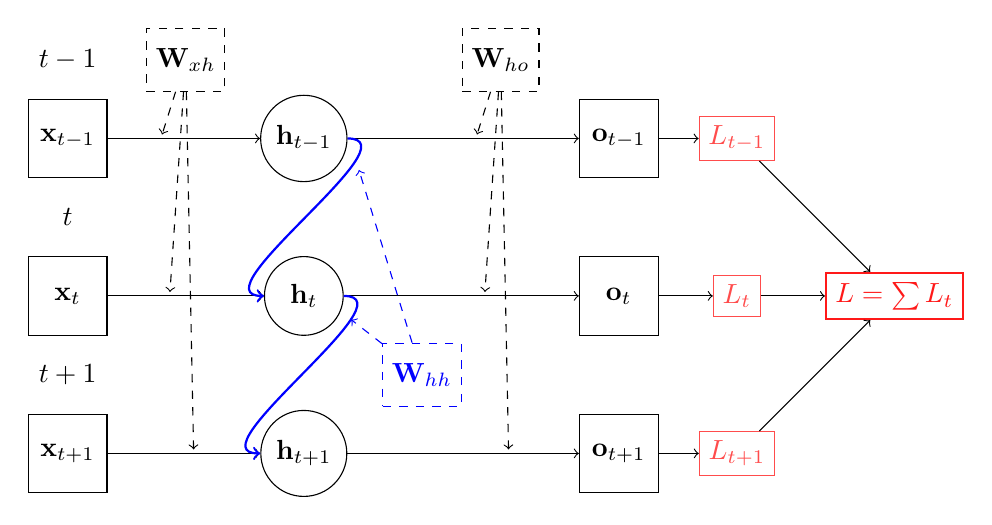
\begin{tikzpicture}[
        node distance=2cm,
        neuron/.style={circle, draw, minimum size=1cm},
        input/.style={rectangle, draw, minimum size=1cm},
        param/.style={rectangle, draw, dashed, minimum size=0.8cm},
        param_rec/.style={rectangle, draw, dashed, blue, minimum size=0.8cm}
    ]
        
        % Input nodes
        \node[input] (x1) at (-1,0) {$\mathbf{x}_{t-1}$};
        \node[input] (x2) at (-1,-2) {$\mathbf{x}_t$};
        \node[input] (x3) at (-1,-4) {$\mathbf{x}_{t+1}$};
        
        % Hidden states
        \node[neuron] (h0) at (2,0) {$\mathbf{h}_{t-1}$};
        \node[neuron] (h1) at (2,-2) {$\mathbf{h}_t$};
        \node[neuron] (h2) at (2,-4) {$\mathbf{h}_{t+1}$};
        
        % Outputs
        \node[input] (o1) at (6,0) {$\mathbf{o}_{t-1}$};
        \node[input] (o2) at (6,-2) {$\mathbf{o}_t$};
        \node[input] (o3) at (6,-4) {$\mathbf{o}_{t+1}$};
        
        % Parameters
        \node[param] (Wxh) at (0.5,1) {$\mathbf{W}_{xh}$};
        \node[param_rec] (Whh) at (3.5,-3.0) {$\mathbf{W}_{hh}$};
        \node[param] (Who) at (4.5,1) {$\mathbf{W}_{ho}$};
        
        % Arrows
        \draw[->] (x1) -- (h0);
        \draw[->] (x2) -- (h1);
        \draw[->] (x3) -- (h2);
        
        \draw[->] (h0) -- (o1);
        \draw[->] (h1) -- (o2);
        \draw[->] (h2) -- (o3);
        
        % Parameter connections
        \draw[->, dashed] (Wxh) -- (0.2,0.05);
        \draw[->, dashed] (Wxh) -- (0.3,-1.95);
        \draw[->, dashed] (Wxh) -- (0.6,-3.95);
        \draw[->, dashed, blue] (Whh) -- (2.7,-0.4);
        \draw[->, dashed, blue] (Whh) -- (2.6,-2.3);
        \draw[->, dashed] (Who) -- (4.2,0.05);
        \draw[->, dashed] (Who) -- (4.3,-1.95);
        \draw[->, dashed] (Who) -- (4.6,-3.95);
        
        % Loss functions
        \node[rectangle, draw, red!70] (L1) at (7.5,0) {$L_{t-1}$};
        \node[rectangle, draw, red!70] (L2) at (7.5,-2) {$L_t$};
        \node[rectangle, draw, red!70] (L3) at (7.5,-4) {$L_{t+1}$};
        
        \draw[->] (o1) -- (L1);
        \draw[->] (o2) -- (L2);
        \draw[->] (o3) -- (L3);
        
        % Total loss
        \node[rectangle, draw, thick, red!90] (L) at (9.5,-2) {$L = \sum L_t$};
        \draw[->] (L1) -- (L);
        \draw[->] (L2) -- (L);
        \draw[->] (L3) -- (L);

        % Time labels
        \node at (-1,1) {$t-1$};
        \node at (-1,-1) {$t$};
        \node at (-1,-3) {$t+1$};
        
        % Recurrent connection
        \draw[->, thick, blue] (h0.east) to[out=0, in=180] (h1.west);
        \draw[->, thick, blue] (h1.east) to[out=0, in=180] (h2.west);
        
    \end{tikzpicture}
    \caption{Unfolded Recurrent Neural Network (RNN) with shared parameters across time.
    The blue arrows show the recurrent connections where $\mathbf{W}_{hh}$ is reused at each time step.}
    \label{chain-rule-to-bptt:fig:rnn_unfolded}
\end{figure}

The forward pass for $t=1,\dots,T$ is explicitly given by:
\begin{align*}
    \mathbf{a}_t &= \mathbf{W}_{hh} \mathbf{h}_{t-1} + \mathbf{W}_{xh} \mathbf{x}_t + \mathbf{b}_h \\
    \mathbf{h}_t &= \sigma(\mathbf{a}_t) \\
    \mathbf{o}_t &= \mathbf{W}_{ho} \mathbf{h}_t + \mathbf{b}_o \\
    L_t &= \ell(\mathbf{o}_t, \mathbf{y}_t)
\end{align*}

From the chain rule perspective, we have a composition of functions:
\begin{align*}
    L = \sum_{t=1}^{T} L_t &= \sum_{t=1}^{T} \ell(\mathbf{o}_t(\mathbf{h}_t(\mathbf{h}_{t-1}, \mathbf{x}_t))) \\
    &= \ell(\mathbf{o}_{1}(\mathbf{h}_{1}(\mathbf{h}_{0}, \mathbf{x}_{1}))) + 
    \ell(\mathbf{o}_{2}(\mathbf{h}_{2}(\mathbf{h}_{1}((\mathbf{h}_{0}, \mathbf{x}_{1}), \mathbf{x}_{2})))) + \\
    & \qquad \cdots +
    \ell(\mathbf{o}_T(\mathbf{h}_T(\mathbf{h}_{T-1}, (\cdots ((\mathbf{h}_{0}, \mathbf{x}_{1}), \cdots)),
    \mathbf{x}_{T-1}), \mathbf{x}_{T})) \\
    \mathbf{h}_t &= \sigma(\mathbf{a}_t(\mathbf{h}_{t-1}, \mathbf{x}_t))
\end{align*}

The unfolded representation in Figure \ref{chain-rule-to-bptt:fig:rnn_unfolded} clearly shows:
\begin{enumerate}
    \item Each time step has its own copy of the computation
    \item Parameters $\mathbf{W}_{hh}, \mathbf{W}_{xh}, \mathbf{W}_{ho}$ are \textbf{shared} across all time steps
    \item Hidden state $\mathbf{h}_t$ serves as input to the next time step $\mathbf{h}_{t+1}$
    \item The total loss $L$ is the sum of individual losses $L_t$
\end{enumerate}

This unfolding transforms the recurrent network into what appears to be a
deep feedforward network, allowing us to apply the chain rule systematically
through time.

\subsection{Gradient Computation via BPTT: Chain Rule Application}

Define the \textbf{hidden state gradient} or \textbf{adjoint variable}:
\[
\bm{\delta}_t = \nabla_{\mathbf{h}_t} L =
\left(\frac{\partial L}{\partial \mathbf{h}_t}\right)^\mathsf{T} \in \mathbb{R}^h
\]

Note: Since $L$ is a scalar, $\frac{\partial L}{\partial \mathbf{h}_t}$ is a
$1 \times h$ Jacobian (row vector), and $\nabla_{\mathbf{h}_t} L$ is its
transpose
(column vector).

Since the total loss $L = \sum_{k=1}^\mathsf{T} L_k$ and the hidden state $\mathbf{h}_t$
only influences losses from time $t$ onward (due to the causal structure of
RNNs),
we have:
\[
\bm{\delta}_t = \nabla_{\mathbf{h}_t} \Bigg( \sum_{k=t}^\mathsf{T} L_k \Bigg)
\tag{*}
\]

This important observation simplifies the computation:
$\mathbf{h}_t$ does not affect $L_1, \dots, L_{t-1}$, so only future losses
$L_t, L_{t+1}, \dots, L_T$ contribute to $\bm{\delta}_t$.

\subsubsection{Base Case: Final Time Step $T$}

\begin{figure}[h]
    \centering
    \begin{tikzpicture}[
        node distance=2cm,
        neuron/.style={circle, draw, minimum size=1cm},
        input/.style={rectangle, draw, minimum size=1cm},
        param/.style={rectangle, draw, dashed, minimum size=0.8cm},
        param_rec/.style={rectangle, draw, dashed, blue, minimum size=0.8cm}
    ]
        
        % Hidden states
        %\node[neuron] (h0) at (2,0) {$\mathbf{h}_{T-1}$};
        \node[neuron] (h1) at (2,-2) {$\mathbf{h}_T$};
        
        % Outputs
        \node[input] (o1) at (6,-2) {$\mathbf{o}_T$};
        
        % Parameters
        %\node[param_rec] (Whh) at (3.2,-1.0) {$\mathbf{W}_{hh}$};
        \node[param] (Who) at (4.7,-1.0) {$\mathbf{W}_{ho}$};
        
        \draw[->] (h1) -- (o2);
        
        % Parameter connections
        %\draw[->, dashed, blue] (Whh) -- (2.1,-1.0);
        \draw[->, dashed] (Who) -- (4.7,-2.0);
        
        % Loss functions
        \node[rectangle, draw, red!70] (L1) at (7.5,-2) {$L_T$};
        
        \draw[->] (o1) -- (L1);

        % Total loss
        \node[rectangle, draw, thick, red!90] (L) at (9.5,-2) {$L = \sum L_t$};
        \draw[->] (L1) -- (L);

        % Recurrent connection
        %\draw[->, thick, blue] (h0.east) to[out=0, in=180] (h1.west);
        
    \end{tikzpicture}
    \caption{Final Time Step}
    \label{chain-rule-to-bptt:fig:recursive_gradient}
\end{figure}

At the final time step $T$, equation (*) gives
$\bm{\delta}_T = \nabla_{\mathbf{h}_T} L_T$.
To compute this gradient, we apply the chain rule through the output
$\mathbf{o}_T$.

Using the gradient form of the chain rule:
\[
\bm{\delta}_T = \nabla_{\mathbf{h}_T} L_T = 
\left(\frac{\partial \mathbf{o}_T}{\partial \mathbf{h}_T}\right)^\mathsf{T}
\nabla_{\mathbf{o}_T} L_T
\]
\\
Let's understand each term:
\begin{itemize}[leftmargin=*,itemsep=2pt]
    \item $\nabla_{\mathbf{h}_T} L_T$: gradient of scalar loss w.r.t. $\mathbf{h}_T$
    (column vector)
    \item $\frac{\partial \mathbf{o}_T}{\partial \mathbf{h}_T}$: Jacobian of
    vector $\mathbf{o}_T$ w.r.t. $\mathbf{h}_T$ (matrix)
    \item $\nabla_{\mathbf{o}_T} L_T$: gradient of scalar loss w.r.t. $\mathbf{o}_T$
    (column vector)
\end{itemize}
\empty
The chain rule formula is: \textbf{gradient = Jacobian$^\mathsf{T}$ × gradient}.
\vspace{1em}
\\
Now we compute each term:

\begin{itemize}
    \item \textbf{Jacobian $\frac{\partial \mathbf{o}_T}{\partial \mathbf{h}_T}$}:
    Since $\mathbf{o}_T = \mathbf{W}_{ho} \mathbf{h}_T + \mathbf{b}_o$,
    we compute the Jacobian component-wise.
    \vspace{1em}
    \\
    Writing $\mathbf{W}_{ho} = (w_{ij})$, $\mathbf{h}_T = (h_j)$, and
    $\mathbf{o}_T = (o_i)$, we have:
    \[
    o_i = \sum_{j=1}^h w_{ij} h_j + b_i
    \]
    The $(i,j)$-entry of the Jacobian is:
    \[
    \frac{\partial o_i}{\partial h_j} = w_{ij}
    \]
    Therefore, the Jacobian matrix equals the weight matrix:
    \[
    \frac{\partial \mathbf{o}_T}{\partial \mathbf{h}_T} = \mathbf{W}_{ho}
    \]
    
    \item \textbf{Gradient $\nabla_{\mathbf{o}_T} L_T$}: This is the gradient
    of the scalar loss function with respect to the output vector $\mathbf{o}_T$.
    It depends on the specific loss function $\ell(\cdot, \cdot)$ and is a column
    vector of partial derivatives:
    \[
    \nabla_{\mathbf{o}_T} L_T = \begin{bmatrix} \frac{\partial L_T}{\partial o_{T,1}} \\
        \vdots \\ \frac{\partial L_T}{\partial o_{T,q}} \end{bmatrix}
    \]
\end{itemize}

Therefore, substituting into the chain rule:
\[
\bm{\delta}_T = \mathbf{W}_{ho}^\mathsf{T} \nabla_{\mathbf{o}_T} L_T
\]
\indent Where,
\[
L_T = 
\ell(\mathbf{o}_T(\mathbf{h}_T(\mathbf{h}_{T-1}, (\cdots ((\mathbf{h}_{0}, \mathbf{x}_{1}), \cdots)),
    \mathbf{x}_{T-1}), \mathbf{x}_{T}))
\]
\\
%~~~~~~~~~~~~~~~~~~~~~~~~~~~~~~~~~~~~~~~~~~~~~~~~~~~
\indent Let's write it for $T = 3$ (Figure \ref{chain-rule-to-bptt:fig:rnn_T3}): 
$
L_{3} = 
\ell\Bigg(\mathbf{o}_{3}\bigg(\mathbf{h}_{3}\Big(\mathbf{h}_{2}\big(\mathbf{h}_{1}
    (\mathbf{h}_{0}, \mathbf{x}_{1}), \mathbf{x}_{2}\big), \mathbf{x}_{3}\Big)\bigg)\Bigg)
$

\begin{figure}[h]
    \centering
    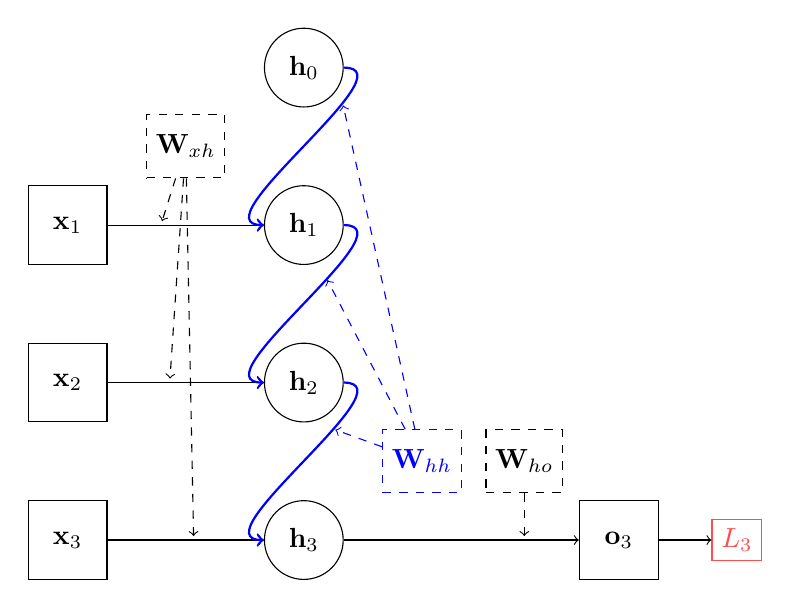
\begin{tikzpicture}[
        node distance=2cm,
        neuron/.style={circle, draw, minimum size=1cm},
        input/.style={rectangle, draw, minimum size=1cm},
        param/.style={rectangle, draw, dashed, minimum size=0.8cm},
        param_rec/.style={rectangle, draw, dashed, blue, minimum size=0.8cm}
    ]
        
        % Input nodes
        \node[input] (x1) at (-1,0) {$\mathbf{x}_{1}$};
        \node[input] (x2) at (-1,-2) {$\mathbf{x}_{2}$};
        \node[input] (x3) at (-1,-4) {$\mathbf{x}_{3}$};
        
        % Hidden states
        \node[neuron] (h0) at (2,2) {$\mathbf{h}_{0}$};
        \node[neuron] (h1) at (2,0) {$\mathbf{h}_{1}$};
        \node[neuron] (h2) at (2,-2) {$\mathbf{h}_{2}$};
        \node[neuron] (h3) at (2,-4) {$\mathbf{h}_{3}$};
        
        % Outputs
        \node[input] (o3) at (6,-4) {$\mathbf{o}_{3}$};
        
        % Parameters
        \node[param] (Wxh) at (0.5,1) {$\mathbf{W}_{xh}$};
        \node[param_rec] (Whh) at (3.5,-3.0) {$\mathbf{W}_{hh}$};
        \node[param] (Who) at (4.8,-3) {$\mathbf{W}_{ho}$};
        
        % Arrows
        \draw[->] (x1) -- (h1);
        \draw[->] (x2) -- (h2);
        \draw[->] (x3) -- (h3);
        
        \draw[->] (h3) -- (o3);
        
        % Parameter connections
        \draw[->, dashed] (Wxh) -- (0.2,0.05);
        \draw[->, dashed] (Wxh) -- (0.3,-1.95);
        \draw[->, dashed] (Wxh) -- (0.6,-3.95);
        \draw[->, dashed, blue] (Whh) -- (2.5,1.52);
        \draw[->, dashed, blue] (Whh) -- (2.3,-0.7);
        \draw[->, dashed, blue] (Whh) -- (2.4,-2.6);
        \draw[->, dashed] (Who) -- (4.8,-3.95);
        
        % Loss functions
        \node[rectangle, draw, red!70] (L3) at (7.5,-4) {$L_{3}$};
        
        \draw[->] (o3) -- (L3);
        
        % Recurrent connection
        \draw[->, thick, blue] (h0.east) to[out=0, in=180] (h1.west);
        \draw[->, thick, blue] (h1.east) to[out=0, in=180] (h2.west);
        \draw[->, thick, blue] (h2.east) to[out=0, in=180] (h3.west);
        
    \end{tikzpicture}
    \caption{$L_{3}$}
    \label{chain-rule-to-bptt:fig:rnn_T3}
\end{figure}

%~~~~~~~~~~~~~~~~~~~~~~~~~~~~~~~~~~~~~~~~~~~~~~~~~~~
\subsubsection{Recursive Case: Time Step $t < T$}

\begin{figure}[h]
    \centering
    \begin{tikzpicture}[
        node distance=2cm,
        neuron/.style={circle, draw, minimum size=1cm},
        input/.style={rectangle, draw, minimum size=1cm},
        param/.style={rectangle, draw, dashed, minimum size=0.8cm},
        param_rec/.style={rectangle, draw, dashed, blue, minimum size=0.8cm}
    ]
        
        % Hidden states
        \node[neuron] (h1) at (2,-2) {$\mathbf{h}_t$};
        \node[neuron] (h2) at (2,-4) {$\mathbf{h}_{t+1}$};
        
        % Outputs
        \node[input] (o2) at (6,-2) {$\mathbf{o}_t$};
        \node[input] (o3) at (6,-4) {$\mathbf{o}_{t+1}$};
        
        % Parameters
        \node[param_rec] (Whh) at (3.2,-3.0) {$\mathbf{W}_{hh}$};
        \node[param] (Who) at (4.7,-3) {$\mathbf{W}_{ho}$};
        
        \draw[->] (h1) -- (o2);
        \draw[->] (h2) -- (o3);
        
        % Parameter connections
        \draw[->, dashed, blue] (Whh) -- (2.0,-3);
        \draw[->, dashed] (Who) -- (4.7,-2.05);
        \draw[->, dashed] (Who) -- (4.7,-3.95);
        
        % Loss functions
        \node[rectangle, draw, red!70] (L2) at (7.5,-2) {$L_t$};
        \node[rectangle, draw, red!70] (L3) at (7.5,-4) {$L_{t+1}$};
        
        \draw[->] (o2) -- (L2);
        \draw[->] (o3) -- (L3);
        
        % 1. Vertical dots below (indicates more steps)
        \node[below=0.5cm of L3] (dots) {\Large $\vdots$};

        % Total loss
        \node[rectangle, draw, thick, red!90] (L) at (9.5,-2) {$L = \sum L_t$};
        \draw[->] (L2) -- (L);
        \draw[->] (L3) -- (L);

        % 3. Arrow from dots to error
        \draw[->, dashed] (dots.east) -- (L);

        % Recurrent connection
        \draw[->, thick, blue] (h1.east) to[out=0, in=180] (h2.west);
        
    \end{tikzpicture}
    \caption{Recursive gradient: the hidden state $\mathbf{h}_t$ influences the loss directly and through $\mathbf{h}_{t+1}$}
    \label{chain-rule-to-bptt:fig:recursive_gradient_unrolled}
\end{figure}

For $t < T$, $\mathbf{h}_t$ influences the loss in two ways:
\begin{enumerate}
    \item \textbf{Directly} through the output $\mathbf{o}_t$ at time $t$
    \item \textbf{Indirectly} through the next hidden state $\mathbf{h}_{t+1}$, which then affects all future losses
\end{enumerate}

For example, at $T-1$, applying the chain rule to account for both contributions to (*) yields:
\begin{align*}
    \bm{\delta}_{T-1} &= \nabla_{\mathbf{h}_{T-1}} \left( L_{T-1} + L_{T} \right) \\
    &= \nabla_{\mathbf{h}_{T-1}} L_{T-1} + \nabla_{\mathbf{h}_{T-1}} L_{T} \\
    &= \nabla_{\mathbf{h}_{T-1}} L_{T-1} + \underbrace{\left(\frac{\partial \mathbf{h}_{T}}
    {\partial \mathbf{h}_{T-1}}\right)^\mathsf{T} \nabla_{\mathbf{h}_{T}}
    L_{T}}_{\text{(chain rule)}} \\
    &= \left(\frac{\partial \mathbf{o}_t}{\partial \mathbf{h}_{T-1}}\right)^\mathsf{T}
    \nabla_{\mathbf{o}_{T-1}} L_{T-1} + \left(\frac{\partial \mathbf{h}_{T}}{\partial
    \mathbf{h}_{T-1}}\right)^\mathsf{T} \bm{\delta}_{T}
\end{align*}

More generaly:
\begin{align*}
    \bm{\delta}_t &= \nabla_{\mathbf{h}_t} \left( L_t + \sum_{k=t+1}^{T} L_k \right) \\
    &= \nabla_{\mathbf{h}_t} L_t + \nabla_{\mathbf{h}_t} \sum_{k=t+1}^{T} L_k \\
    &= \nabla_{\mathbf{h}_t} L_t +
    \underbrace{\left(\frac{\partial \mathbf{h}_{t+1}}{\partial \mathbf{h}_t}\right)^\mathsf{T} 
    \nabla_{\mathbf{h}_{t+1}} \sum_{k=t+1}^{T} L_k}_{\text{(chain rule)}} \\
    &= \left(\frac{\partial \mathbf{o}_t}{\partial \mathbf{h}_t}\right)^\mathsf{T}
    \nabla_{\mathbf{o}_t} L_t + \left(\frac{\partial \mathbf{h}_{t+1}}{\partial
    \mathbf{h}_t}\right)^\mathsf{T} \bm{\delta}_{t+1}
\end{align*}

Now compute the Jacobians:
\begin{align*}
    \frac{\partial \mathbf{o}_t}{\partial \mathbf{h}_t} &= \mathbf{W}_{ho} \quad \text{(same reasoning as for $\mathbf{o}_T$)} \\
\frac{\partial \mathbf{h}_{t+1}}{\partial \mathbf{h}_t} &=
\frac{\partial}{\partial \mathbf{h}_t} \sigma(\mathbf{a}_{t+1})
    = \frac{\partial \sigma(\mathbf{a}_{t+1})}{\partial \mathbf{a}_{t+1}} \cdot
      \frac{\partial \mathbf{a}_{t+1}}{\partial \mathbf{h}_t}
      \quad \text{(chain rule through $\sigma$)}\\
&= J_{\sigma}(\mathbf{a}_{t+1}) \cdot \frac{\partial \mathbf{a}_{t+1}}{\partial
\mathbf{h}_t}
\end{align*}
%
\begin{equation*}
\text{where } J_{\sigma}(\mathbf{a}_{t+1}) = \begin{bmatrix}
\frac{\partial \sigma(a_1)}{\partial a_1} & \frac{\partial \sigma(a_1)}{\partial a_2} & \cdots & \frac{\partial \sigma(a_1)}{\partial a_m} \\
\frac{\partial \sigma(a_2)}{\partial a_1} & \frac{\partial \sigma(a_2)}{\partial a_2} & \cdots & \frac{\partial \sigma(a_2)}{\partial a_m} \\
\vdots & \vdots & \ddots & \vdots \\
\frac{\partial \sigma(a_m)}{\partial a_1} & \frac{\partial \sigma(a_m)}{\partial
n_2} & \cdots & \frac{\partial \sigma(a_m)}{\partial a_m}
\end{bmatrix}
= \begin{bmatrix}
\sigma'(a_1) & 0 & \cdots & 0 \\
0 & \sigma'(a_2) & \cdots & 0 \\
\vdots & \vdots & \ddots & \vdots \\
0 & 0 & \cdots & \sigma'(a_m)
\end{bmatrix}
\end{equation*}
%
\begin{align*}
    \text{Therefore, } \quad
    \frac{\partial \mathbf{h}_{t+1}}{\partial \mathbf{h}_t} &=
    \text{diag}(\sigma'(\mathbf{a}_{t+1})) \frac{\partial \mathbf{a}_{t+1}}{\partial \mathbf{h}_t} \\
&= \text{diag}(\sigma'(\mathbf{a}_{t+1})) \mathbf{W}_{hh} \quad \text{(since
$\mathbf{a}_{t+1} = \mathbf{W}_{hh}\mathbf{h}_t +
\mathbf{W}_{xh}\mathbf{x}_{t+1} + \mathbf{b}_h$)}
\end{align*}

Finally, we obtain the backward recurrence:
\begin{align*}
    \bm{\delta}_t &= \mathbf{W}_{ho}^\mathsf{T} \nabla_{\mathbf{o}_t} L_t + \mathbf{W}_{hh}^\mathsf{T} \text{diag}(\sigma'(\mathbf{a}_{t+1})) \bm{\delta}_{t+1} \\
&= \mathbf{W}_{ho}^\mathsf{T} \nabla_{\mathbf{o}_t} L_t + \mathbf{W}_{hh}^\mathsf{T} \left(
\bm{\delta}_{t+1} \odot \sigma'(\mathbf{a}_{t+1}) \right)
\end{align*}
where $\odot$ denotes element-wise multiplication.

\begin{keyinsight}[title=The Recursive Structure of BPTT]
This backward recurrence is the heart of BPTT. Notice that:
\begin{enumerate}[itemsep=0pt]
    \item We compute $\bm{\delta}_t$ from $\bm{\delta}_{t+1}$ (backward in time)
    \item At each step, we combine the \textbf{direct contribution} ($\mathbf{W}_{ho}^\mathsf{T} \nabla_{\mathbf{o}_t} L_t$) with the \textbf{indirect contribution} ($\mathbf{W}_{hh}^\mathsf{T} (\bm{\delta}_{t+1} \odot \sigma'(\mathbf{a}_{t+1}))$)
    \item The indirect contribution propagates gradients from all future time steps
\end{enumerate}
This is exactly analogous to backpropagation in feedforward networks, but
unfolded through time rather than through layers. The key difference is that the
same weight matrix $\mathbf{W}_{hh}$ appears at every time step!
\end{keyinsight}

This recurrence shows that $\bm{\delta}_t$ depends on:
\begin{itemize}
    \item The current output gradient $\nabla_{\mathbf{o}_t} L_t$
    \item The next hidden state gradient $\bm{\delta}_{t+1}$
    \item The weight matrices $\mathbf{W}_{ho}$ and $\mathbf{W}_{hh}$
    \item The activation derivative $\sigma'(\mathbf{a}_{t+1})$
\end{itemize}

\subsection{Parameter Gradients via Chain Rule: Detailed Derivations}

For parameters that appear at multiple time steps (like $\mathbf{W}_{hh}$,
$\mathbf{W}_{xh}$, and $\mathbf{b}_h$), we need to sum contributions from
all time steps where they are used.
Let's derive each gradient systematically using the chain rule.
%=================================================================
% Gradient for W_hh
%=================================================================
\subsubsection{Gradient for $\mathbf{W}_{hh}$}

To compute $\frac{\partial L}{\partial \mathbf{W}_{hh}}$, we need to understand
what it means to differentiate with respect to a matrix. We'll start at the most
fundamental level—computing individual elements—then build up to tensor and
matrix forms.

\paragraph{Part 1:}\textbf{Element-wise derivation}

\vspace{1em}
\textbf{Step 1: Single weight element perspective}
\vspace{1em}

Focus on one specific weight $(W_{hh})_{kl}$ (row $k$, column $l$). Since
$\mathbf{W}_{hh}$ appears at every time step $t = 1, \dots, T$, this weight
affects the loss $L$ through all pre-activations $\mathbf{a}_1, \dots,
\mathbf{a}_T$.

By the multivariable chain rule:
\[
\frac{\partial L}{\partial (W_{hh})_{kl}} = \sum_{t=1}^{T} \sum_{i=1}^{m} \frac{\partial L}{\partial a_{t,i}} \cdot \frac{\partial a_{t,i}}{\partial (W_{hh})_{kl}}
\tag{W.1}
\]

This sums over all paths: $(W_{hh})_{kl} \rightarrow a_{t,i} \rightarrow L$.

\vspace{1em}
\textbf{Step 2: Compute $\frac{\partial a_{t,i}}{\partial (W_{hh})_{kl}}$}
\vspace{1em}

From $\mathbf{a}_t = \mathbf{W}_{hh} \mathbf{h}_{t-1} + \mathbf{W}_{xh}
\mathbf{x}_t + \mathbf{b}_h$, the $i$-th component is:
\[
a_{t,i} = \sum_{j=1}^{m} (W_{hh})_{ij} (h_{t-1})_j + \text{(terms independent of $(W_{hh})_{kl}$)}
\]

The derivative is:
\[
\frac{\partial a_{t,i}}{\partial (W_{hh})_{kl}} = 
\begin{cases}
(h_{t-1})_l & \text{if } i = k \\
0 & \text{if } i \neq k
\end{cases}
\]

Using the Kronecker delta $\delta_{ik}$:
\[
\frac{\partial a_{t,i}}{\partial (W_{hh})_{kl}} = \delta_{ik} (h_{t-1})_l
\tag{W.2}
\]

\vspace{1em}
\textbf{Step 3: Substitute into (W.1)}
\vspace{1em}

Plug (W.2) into (W.1):
\[
\frac{\partial L}{\partial (W_{hh})_{kl}} =
\sum_{t=1}^{T} \sum_{i=1}^{m} \frac{\partial L}{\partial a_{t,i}}
\cdot \delta_{ik} (h_{t-1})_l
\]

The Kronecker delta collapses the sum over $i$:
\[
\boxed{\frac{\partial L}{\partial (W_{hh})_{kl}} =
\sum_{t=1}^{T} \frac{\partial L}{\partial a_{t,k}} \cdot (h_{t-1})_l}
\tag{W.3}
\]

\textbf{Interpretation:} The Jacobian for weight $(k,l)$ is:
\begin{itemize}
    \item For each time $t$, take $\frac{\partial L}{\partial a_{t,k}}$
    (how $L$ changes with the $k$-th component of $\mathbf{a}_t$)
    \item Multiply by $(h_{t-1})_l$ (the $l$-th component of the previous hidden state)
    \item Sum over all time steps
\end{itemize}

\paragraph{Part 2:}\textbf{From elements to tensor structure}

\vspace{1em}
\textbf{Step 4: Organize all derivatives into a tensor}
\vspace{1em}

For each time $t$, consider all partial derivatives
$\frac{\partial a_{t,i}}{\partial (W_{hh})_{kl}}$.\\

These form a third-order tensor $\frac{\partial \mathbf{a}_t}{\partial
\mathbf{W}_{hh}}$
with dimensions $(m, m, m)$:
\begin{itemize}
    \item First dimension $i$: component of $\mathbf{a}_t$ ($i = 1, \dots, m$)
    \item Second dimension $k$: row of $\mathbf{W}_{hh}$ ($k = 1, \dots, m$)
    \item Third dimension $l$: column of $\mathbf{W}_{hh}$ ($l = 1, \dots, m$)
\end{itemize}

From (2), each element is:
\[
\left(\frac{\partial \mathbf{a}_t}{\partial \mathbf{W}_{hh}}\right)_{i,k,l} = \delta_{ik} (h_{t-1})_l
\]
%========================================================================

%========================================================================
\vspace{1em}
\textbf{Step 5: Visualize the tensor}
\vspace{1em}

Fix indices $k$ and $l$ (one specific weight). We get an $m \times 1$ vector:
\[
\frac{\partial \mathbf{a}_t}{\partial (W_{hh})_{kl}} = \quad
\begin{bNiceMatrix}[first-col, margin]
$i = 1$      & 0 \\
\Vdots & \Vdots \\
$i = k-1$    & 0 \\
$i = k$      & (h_{t-1})_l \\
$i = k+1$    & 0 \\
\Vdots & \Vdots \\
$i = m$      & 0 
\end{bNiceMatrix}
= (h_{t-1})_l \mathbf{e}_k
\]
\indent where $\mathbf{e}_k$ is the $k$-th standard basis column vector.

Thus, for a given $k$ \it{(a row of $\mathbf{W}_{hh}$)} we have the $m \times m$
matrix:
\[
\frac{\partial \mathbf{a}_t}{\partial (W_{hh})_{k\bullet}} = 
\begin{bNiceMatrix}[first-col, first-row, margin]
       & 1      &        & l      &        & m      \\
1      & 0      & \Cdots & 0      & \Cdots & 0      \\
\Vdots & \Vdots & \Ddots & \Vdots & \Ddots & \Vdots \\
k-1    & 0      & \Cdots & 0      & \Cdots & 0      \\
k      & (h_{t-1})_1 & \Cdots & (h_{t-1})_l & \Cdots & (h_{t-1})_m \\
k+1    & 0      & \Cdots & 0      & \Cdots & 0      \\
\Vdots & \Vdots & \Ddots & \Vdots & \Ddots & \Vdots \\
m      & 0      & \Cdots & 0      & \Cdots & 0      
\end{bNiceMatrix}
= \mathbf{e}_k \mathbf{h}_{t-1}^\mathsf{T}
\]

The full tensor \(\frac{\partial \mathbf{a}_t}{\partial \mathbf{W}_{hh}}\) is an
\(m \times m \times m\) array. Each "slice" (fixed \(i\)) is an \(m \times m\)
matrix showing \(\frac{\partial a_{t,i}}{\partial \mathbf{W}_{hh}}\).

\medskip

\begin{center}
\begin{tikzpicture}[scale=1.2]
    % Define the three matrices with proper 3D spacing
    % Bottom-left corner coordinates for each matrix
    \def\xfront{0}
    \def\yfront{0}
    
    \def\xmid{2.8}
    \def\ymid{2.8}
    
    \def\xback{5.5}
    \def\yback{5.5}
    
    % Matrix dimensions
    \def\matwidth{3}
    \def\matheight{3}
    
    % ----- Draw the back matrix (i=m) -----
    \node[rectangle, inner sep=0pt, opacity=0.6] (back) at (\xback,\yback) {%
        $\begin{bNiceMatrix}
        0 & 0 & \Cdots & 0 \\
        \Vdots & \Vdots & \Ddots & \Vdots \\
        0 & 0 & \Cdots & 0 \\
        (h_{t-1})_1 & (h_{t-1})_2 & \Cdots & (h_{t-1})_m
        \end{bNiceMatrix}$
    };
\node[font=\scriptsize] at ($(back.east) + (0.45, 0.95)$)
{\(\textcolor{blue}{i=m}\)};
    
    % ----- Draw the middle matrix (i=k) -----
    \node[rectangle, inner sep=0pt, opacity=0.8] (middle) at (\xmid,\ymid) {%
        $\begin{bNiceMatrix}
        0 & 0 & \Cdots & 0 \\
        \Vdots & \Vdots & \Ddots & \Vdots \\
        (h_{t-1})_1 & (h_{t-1})_2 & \Cdots & (h_{t-1})_m \\
        \Vdots & \Vdots & \Ddots & \Vdots \\
        0 & 0 & \Cdots & 0
        \end{bNiceMatrix}$
    };
\node[font=\scriptsize] at ($(middle.east) + (0.5, 1.1)$)
{\(\textcolor{blue}{i=k}\)};
    
    % ----- Draw the front matrix (i=1) -----
    \node[rectangle, inner sep=0pt, opacity=1.0] (front) at (\xfront,\yfront) {%
        $\begin{bNiceMatrix}
        (h_{t-1})_1 & (h_{t-1})_2 & \Cdots & (h_{t-1})_m \\
        0 & 0 & \Cdots & 0 \\
        \Vdots & \Vdots & \Ddots & \Vdots \\
        0 & 0 & \Cdots & 0
        \end{bNiceMatrix}$
    };
\node[font=\scriptsize] at ($(front.east) + (0.2, 0.95)$)
{\(\textcolor{blue}{i=1}\)};
    
    % ----- Draw connecting lines for 3D effect -----
    \draw[dotted, gray!50] (back.north west) -- (front.north west);
    \draw[dotted, gray!50] (back.north east) -- (front.north east);
    \draw[dotted, gray!50] (back.south west) -- (front.south west);
    \draw[dotted, gray!50] (back.south east) -- (front.south east);
    
    % ----- Add dimension labels -----
    % X-axis (columns, l dimension)
    \draw[->, thick, red!70] ($(front.south east)+(-4.2,-0.2)$) -- 
        node[midway, below, font=\tiny] {\(l\) (columns)} 
        ($(front.south east)+(-0.5,-0.2)$);
    
    % Y-axis (rows, k dimension)  
    \draw[->, thick, green!70] ($(front.north west)+(-0.2,-0.1)$) -- 
        node[midway, left, font=\tiny, align=right] {\(k\)\\ (rows)} 
        ($(front.north west)+(-0.2,-1.8)$);
    
    % Z-axis (depth, i dimension)
    \draw[->, thick, blue!70] ($(front.north east)+(0.1,0.1)$) -- 
        node[midway, above right, font=\tiny, sloped] {\(i\) (slices)} 
        ($(back.north east)+(0.1,0.1)$);
    
    % ----- Add a legend -----
\node[right=1.5cm of front.east, font=\scriptsize, align=left, text width=4cm]
(legend) {
        \textbf{Tensor Structure:}\\
        Dimensions: \(m \times m \times m\)\\
        Each slice \(i\):\\
        - Only row \(k=i\) nonzero\\
        - Entries: \((h_{t-1})_1, \dots, (h_{t-1})_m\)\\
        - All other rows: zero\\
        \vspace{2pt}
        Sparse: \(m^2\) of \(m^3\) entries are non-zero
    };
    
\end{tikzpicture}
\end{center}

Which we can write in a more compact way as a $m \times m$ matrix of vectors:

\[
\frac{\partial \mathbf{a}_t}{\partial \mathbf{W}_{hh}} = 
\begin{bNiceMatrix}[first-row, first-col]
       & \text{Col }1 & \cdots & \text{Col }\textcolor{red}{l} & \cdots & \text{Col }m \\
\text{Row }1 & 
(h_{t-1})_1 \mathbf{e}_1 & \cdots & 
(h_{t-1})_{\textcolor{red}{l}} \mathbf{e}_1 & \cdots & 
(h_{t-1})_m \mathbf{e}_1 \\
\vdots & \vdots & \ddots & \vdots & \ddots & \vdots \\
\text{Row }\textcolor{blue}{k} & 
(h_{t-1})_1 \mathbf{e}_{\textcolor{blue}{k}} & \cdots & 
(h_{t-1})_{\textcolor{red}{l}} \mathbf{e}_{\textcolor{blue}{k}} & \cdots & 
(h_{t-1})_m \mathbf{e}_{\textcolor{blue}{k}} \\
\vdots & \vdots & \ddots & \vdots & \ddots & \vdots \\
\text{Row }m & 
(h_{t-1})_1 \mathbf{e}_m & \cdots & 
(h_{t-1})_{\textcolor{red}{l}} \mathbf{e}_m & \cdots & 
(h_{t-1})_m \mathbf{e}_m
\end{bNiceMatrix}
\]

\begin{keyinsight}[title=Understanding the Tensor Structure]
The 3D tensor $\frac{\partial \mathbf{a}_t}{\partial \mathbf{W}_{hh}}$
has dimensions $(m \times m \times m)$, but it's \textbf{highly sparse}:
\begin{itemize}[itemsep=0pt]
    \item Only $m^2$ out of $m^3$ entries are non-zero
    \item For each "slice" $i$, only row $k=i$ is non-zero
    \item This sparsity pattern arises because each component $a_{t,i}$
    depends only on row $i$ of $\mathbf{W}_{hh}$
\end{itemize}
This sparse structure is why we can efficiently express the gradient as
an outer product instead of storing the full 3D tensor!
\end{keyinsight}

\vspace{1em}
\textbf{Step 6: The chain rule for tensors}
\vspace{1em}

Now we understand what $\frac{\partial \mathbf{a}_t}{\partial \mathbf{W}_{hh}}$
means.
The chain rule for the full Jacobian matrix is:
\[
\frac{\partial L}{\partial \mathbf{W}_{hh}} =
\sum_{t=1}^{T} \frac{\partial L}{\partial \mathbf{a}_t} \frac{\partial \mathbf{a}_t}{\partial \mathbf{W}_{hh}}
\tag{W.4}
\]

\textbf{What does $\frac{\partial L}{\partial \mathbf{a}_t} \frac{\partial
\mathbf{a}_t}
{\partial \mathbf{W}_{hh}}$ mean?}
\begin{itemize}
    \item $\frac{\partial L}{\partial \mathbf{a}_t}$ is an $1 \times m$ row vector:
    $
        \frac{\partial L}{\partial \mathbf{a}_t} = 
        \begin{bmatrix}
            \frac{\partial L}{\partial a_{t,1}} & 
            \frac{\partial L}{\partial a_{t,2}} &
            \cdots &
            \frac{\partial L}{\partial a_{t,m}}
        \end{bmatrix}
    $
    \item $\frac{\partial \mathbf{a}_t}{\partial \mathbf{W}_{hh}}$ is an
    $m \times m \times m$ tensor ($m$ slices of $m \times m$ matrices)
    \item The product contracts over the $i$ index (component of $\mathbf{a}_t$):\\
    You multiply the first scalar of the vector by the first matrix slice,
    the second scalar by the second slice, and so on.
    Summing all these scaled matrices produces the final resultant matrix.
\end{itemize}

Explicitly, for time step $t$ element $(k,l)$ of the resultant matrix is given
by:
\[
\left(\frac{\partial L}{\partial \mathbf{W}_{hh}}\right)_{kl} = 
\sum_{i=1}^m \left(\frac{\partial L}{\partial \mathbf{a}_t}\right)_i 
\cdot \left(\frac{\partial \mathbf{a}_t}{\partial \mathbf{W}_{hh}}\right)_{i,k,l}
\]

Substitute $\left(\frac{\partial \mathbf{a}_t}{\partial
\mathbf{W}_{hh}}\right)_{i,k,l} = \delta_{ik} (h_{t-1})_l$:
\[
\left(\frac{\partial L}{\partial \mathbf{W}_{hh}}\right)_{kl} = 
\sum_{i=1}^m \left(\frac{\partial L}{\partial \mathbf{a}_t}\right)_i \delta_{ik} (h_{t-1})_l
= \left(\frac{\partial L}{\partial \mathbf{a}_t}\right)_k (h_{t-1})_l
\]

Summing over $t$ gives exactly equation (3), showing consistency.

\paragraph{Part 3:}\textbf{From tensor to matrix form}

\vspace{1em}
\textbf{Step 7: Recognize the pattern in (3)}
\vspace{1em}

Equation (3) shows each gradient element is a sum of products $\frac{\partial
L}{\partial a_{t,k}} \cdot (h_{t-1})_l$.

Recall that $\frac{\partial L}{\partial \mathbf{a}_t}$ is the Jacobian (1×m row
vector):
\[
\frac{\partial L}{\partial \mathbf{a}_t} = 
\begin{bmatrix}
\frac{\partial L}{\partial a_{t,1}} &
\frac{\partial L}{\partial a_{t,2}} &
\cdots &
\frac{\partial L}{\partial a_{t,m}}
\end{bmatrix}_{1 \times m}
\]

And $\mathbf{h}_{t-1}$ is a column vector:
\[
\mathbf{h}_{t-1} =
\begin{bmatrix} (h_{t-1})_1 \\ (h_{t-1})_2 \\ \vdots \\ (h_{t-1})_m \end{bmatrix}_{m \times 1}
\]

To get entry $(k,l) = \frac{\partial L}{\partial a_{t,k}} \cdot (h_{t-1})_l$, we
need the outer product of the \textbf{gradient} (transpose of Jacobian) with the
transposed hidden state:
\[
\left(\frac{\partial L}{\partial \mathbf{a}_t}\right)^\mathsf{T} \mathbf{h}_{t-1}^\mathsf{T}
= (m \times 1) \times (1 \times m) = m \times m
\]

where entry $(k,l)$ is exactly $\frac{\partial L}{\partial a_{t,k}} \cdot
(h_{t-1})_l$.

Thus:
\[
\frac{\partial L}{\partial \mathbf{W}_{hh}} =
\sum_{t=1}^{T} \left(\frac{\partial L}{\partial \mathbf{a}_t}\right)^\mathsf{T} \mathbf{h}_{t-1}^\mathsf{T}
\tag{W.5}
\]

\vspace{1em}
\textbf{Step 8: Connect to backpropagation variables}
\vspace{1em}

From earlier derivations, $\bm{\delta}_t = \nabla_{\mathbf{h}_t} L$ is the
gradient (column vector).

The Jacobian of $L$ with respect to $\mathbf{a}_t$ is:
\[
    \frac{\partial L}{\partial \mathbf{a}_t} =
    \frac{\partial L}{\partial \mathbf{h}_t}
    \frac{\partial \mathbf{h}_t}{\partial \mathbf{a}_t} =
    \frac{\partial L}{\partial \mathbf{h}_t} \text{diag}(\sigma'(\mathbf{a}_t))
\]

Since $\frac{\partial L}{\partial \mathbf{h}_t} = \bm{\delta}_t^\mathsf{T}$ (Jacobian =
gradient transposed), and using element-wise multiplication with the diagonal
matrix:
\[
    \frac{\partial L}{\partial \mathbf{a}_t} =
    \bm{\delta}_{t}^{T} \odot \sigma'(\mathbf{a}_t)
    \quad \text{(1×m row vector)}
\]

Taking the transpose:
\[
    \left(\frac{\partial L}{\partial \mathbf{a}_t}\right)^\mathsf{T} =
    \bm{\delta}_{t} \odot \sigma'(\mathbf{a}_t)
    \quad \text{(m×1 column vector)}
\]

Substituting into (W.5):
\begin{equation}
\boxed{\frac{\partial L}{\partial \mathbf{W}_{hh}} =
\sum_{t=1}^{T} (\bm{\delta}_t \odot \sigma'(\mathbf{a}_t)) 
\mathbf{h}_{t-1}^\mathsf{T}}
\label{chain-rule-to-bptt:eq:dWhh_detailed}
\end{equation}
\\
\textbf{Summary of the derivation path:}
\begin{enumerate}
    \item \textbf{Element-wise:} Start with single weight $(W_{hh})_{kl}$ → chain rule gives equation (W.3)
    \item \textbf{Tensor view:} Organize all derivatives into $\frac{\partial \mathbf{a}_t}{\partial \mathbf{W}_{hh}}$ → understand tensor contraction in chain rule (W.4)
    \item \textbf{Matrix form:} Recognize outer product pattern → obtain compact matrix formula (W.5)
    \item \textbf{Final expression:} Substitute backpropagation variables → get practical formula (\ref{chain-rule-to-bptt:eq:dWhh_detailed})
\end{enumerate}

%=================================================================
% Derivations checked and corrected
%================================================================
\subsubsection{Gradient for $\mathbf{W}_{xh}$}

The derivation for $\mathbf{W}_{xh}$ follows similar steps. The matrix
$\mathbf{W}_{xh}$ appears in $\mathbf{a}_t = \mathbf{W}_{hh} \mathbf{h}_{t-1} +
\mathbf{W}_{xh} \mathbf{x}_t + \mathbf{b}_h$.\\

Using the chain rule:
\begin{align*}
    \frac{\partial L}{\partial \mathbf{W}_{xh}} 
&= \sum_{t=1}^{T} \frac{\partial L}{\partial \mathbf{a}_t} \frac{\partial
\mathbf{a}_t}{\partial \mathbf{W}_{xh}}
\end{align*}

From the previous derivation: $\frac{\partial L}{\partial \mathbf{a}_t} =
\bm{\delta}_t^\mathsf{T} \odot \sigma'(\mathbf{a}_t)$ (1×m row vector).
\vspace{1em}
\\
\indent For $\frac{\partial \mathbf{a}_t}{\partial \mathbf{W}_{xh}}$, we compute
component-wise:
\[
a_{t,i} = \sum_{j=1}^d (W_{xh})_{ij} (x_t)_j + \text{(terms not involving $\mathbf{W}_{xh}$)}
\]

The derivative is:
\[
\frac{\partial a_{t,i}}{\partial (W_{xh})_{kl}} = 
\begin{cases}
(x_t)_l & \text{if } i = k \\
0 & \text{if } i \neq k
\end{cases}
\]

Following the same tensor contraction reasoning as for $\mathbf{W}_{hh}$, 
the Jacobian is:
\[
\frac{\partial L}{\partial \mathbf{W}_{xh}} = 
\sum_{t=1}^{T} \left( \frac{\partial L}{\partial \mathbf{a}_t} \right)^\mathsf{T} 
\mathbf{x}_t^\mathsf{T}
\]

where $\left(\frac{\partial L}{\partial \mathbf{a}_t}\right)^\mathsf{T} = 
\bm{\delta}_t \odot \sigma'(\mathbf{a}_t)$ (m×1 column vector) and 
$\mathbf{x}_t^\mathsf{T}$ (1×d row vector), giving an m×d matrix.
%
\begin{align}
\frac{\partial L}{\partial \mathbf{W}_{xh}} &= \sum_{t=1}^{T} \left( \bm{\delta}_t
\odot \sigma'(\mathbf{a}_t) \right) \mathbf{x}_t^\mathsf{T} \label{chain-rule-to-bptt:eq:dWxh_detailed}
\end{align}

\subsubsection{Gradient for $\mathbf{b}_h$}

The bias vector $\mathbf{b}_h$ also appears in every time step. Using the chain
rule:
%
\begin{align*}
    \frac{\partial L}{\partial \mathbf{b}_h} 
&= \sum_{t=1}^{T} \frac{\partial L}{\partial \mathbf{a}_t} \frac{\partial
\mathbf{a}_t}{\partial \mathbf{b}_h}
\end{align*}

From $\mathbf{a}_t = \mathbf{W}_{hh} \mathbf{h}_{t-1} + \mathbf{W}_{xh}
\mathbf{x}_t + \mathbf{b}_h$, we have:
\[
\frac{\partial \mathbf{a}_t}{\partial \mathbf{b}_h} = \mathbf{I}_m \quad 
\text{(the $m \times m$ identity matrix)}
\]

Computing the Jacobian (row vector times identity matrix):
\[
\frac{\partial L}{\partial \mathbf{b}_h} = \sum_{t=1}^{T} \frac{\partial 
L}{\partial \mathbf{a}_t} \mathbf{I}_m
= \sum_{t=1}^{T} \frac{\partial L}{\partial \mathbf{a}_t}
\]

Substituting $\frac{\partial L}{\partial \mathbf{a}_t} = \bm{\delta}_t^\mathsf{T} \odot 
\sigma'(\mathbf{a}_t)$ (1×m row vector):

\begin{align}
\frac{\partial L}{\partial \mathbf{b}_h} &= \sum_{t=1}^{T} \bm{\delta}_t^\mathsf{T} \odot
\sigma'(\mathbf{a}_t) \label{chain-rule-to-bptt:eq:dbh_detailed}
\end{align}

This is the Jacobian (1×m row vector). The corresponding gradient (for use in
gradient descent) is the transpose:
\[
\nabla_{\mathbf{b}_h} L = \left(\frac{\partial L}{\partial \mathbf{b}_h}\right)^\mathsf{T} 
= \sum_{t=1}^{T} \bm{\delta}_t \odot \sigma'(\mathbf{a}_t)
\]

\subsubsection{Gradient for $\mathbf{W}_{ho}$}

The output weight matrix $\mathbf{W}_{ho}$ appears in $\mathbf{o}_t =
\mathbf{W}_{ho} \mathbf{h}_t + \mathbf{b}_o$. Since each loss $L_t$ depends only
on $\mathbf{o}_t$ at time $t$, we have:
%
\begin{align*}
    \frac{\partial L}{\partial \mathbf{W}_{ho}} 
&= \sum_{t=1}^{T} \frac{\partial L_t}{\partial \mathbf{W}_{ho}} \quad \text{(no
cross-time dependencies)}
\end{align*}
%
Using the chain rule through $\mathbf{o}_t$:
\begin{align*}
    \frac{\partial L_t}{\partial \mathbf{W}_{ho}} 
&= \frac{\partial L_t}{\partial \mathbf{o}_t} \frac{\partial
\mathbf{o}_t}{\partial \mathbf{W}_{ho}}
\end{align*}

\noindent Compute $\frac{\partial \mathbf{o}_t}{\partial \mathbf{W}_{ho}}$ component-wise.
\vspace{1em}
\\
For $o_{t,i} = \sum_{j=1}^h (W_{ho})_{ij} (h_t)_j + (b_o)_i$:
\[
\frac{\partial o_{t,i}}{\partial (W_{ho})_{kl}} = 
\begin{cases}
(h_t)_l & \text{if } i = k \\
0 & \text{if } i \neq k
\end{cases}
\]

Following the same pattern, where $\frac{\partial L_t}{\partial \mathbf{o}_t}$
is a 1×q Jacobian (row vector), we get:
\[
\frac{\partial L_t}{\partial \mathbf{W}_{ho}} = \left( \frac{\partial L_t}{\partial \mathbf{o}_t} \right)^\mathsf{T} \mathbf{h}_t^\mathsf{T}
\]

This is (q×1) × (1×m) = q×m matrix, where entry (k,l) = $\frac{\partial
L_t}{\partial o_{t,k}} \times h_{t,l}$.

Using gradient notation, $\nabla_{\mathbf{o}_t} L_t = \left(\frac{\partial
L_t}{\partial \mathbf{o}_t}\right)^\mathsf{T}$:

\begin{align}
\frac{\partial L}{\partial \mathbf{W}_{ho}} &= \sum_{t=1}^{T}
\nabla_{\mathbf{o}_t} L_t \, \mathbf{h}_t^\mathsf{T} \label{chain-rule-to-bptt:eq:dWho_detailed}
\end{align}

\subsubsection{Gradient for $\mathbf{b}_o$}

Similarly, for the output bias $\mathbf{b}_o$:

\begin{align*}
    \frac{\partial L}{\partial \mathbf{b}_o} 
    &= \sum_{t=1}^{T} \frac{\partial L_t}{\partial \mathbf{b}_o} 
= \sum_{t=1}^{T} \frac{\partial L_t}{\partial \mathbf{o}_t} \frac{\partial
\mathbf{o}_t}{\partial \mathbf{b}_o}
\end{align*}

Since $\frac{\partial \mathbf{o}_t}{\partial \mathbf{b}_o} = \mathbf{I}_q$ (the
$q \times q$ identity matrix):
\begin{align}
\frac{\partial L}{\partial \mathbf{b}_o} &= \sum_{t=1}^{T} \frac{\partial 
L_t}{\partial \mathbf{o}_t} \mathbf{I}_q
= \sum_{t=1}^{T} \frac{\partial L_t}{\partial \mathbf{o}_t}
\label{chain-rule-to-bptt:eq:dbo_jacobian}
\end{align}

This is the Jacobian (1×q row vector). The corresponding gradient is:

\begin{align}
\nabla_{\mathbf{b}_o} L &= \left(\frac{\partial L}{\partial 
\mathbf{b}_o}\right)^\mathsf{T} = \sum_{t=1}^{T} \left(\frac{\partial L_t}{\partial 
\mathbf{o}_t}\right)^\mathsf{T}
    = \sum_{t=1}^{T} \nabla_{\mathbf{o}_t} L_t \label{chain-rule-to-bptt:eq:dbo_gradient}
\end{align}

\subsubsection{Summary of Parameter Gradients}

We have derived all parameter Jacobians (derivatives of scalar loss $L$ with
respect to parameters). For matrix parameters, these are simply matrices of
partial derivatives. For vector parameters (biases), the Jacobian is a row
vector, and the gradient (used in updates) is its transpose:

\textbf{Parameter Jacobians:}
\begin{align}
    \frac{\partial L}{\partial \mathbf{W}_{hh}} &= \sum_{t=1}^{T} 
    \left( \bm{\delta}_t \odot \sigma'(\mathbf{a}_t) \right)
    \mathbf{h}_{t-1}^\mathsf{T} \tag{\ref{chain-rule-to-bptt:eq:dWhh_detailed}} \\
    \frac{\partial L}{\partial \mathbf{W}_{xh}} &= 
    \sum_{t=1}^{T} \left( \bm{\delta}_t \odot \sigma'(\mathbf{a}_t) \right)
    \mathbf{x}_t^\mathsf{T} \tag{\ref{chain-rule-to-bptt:eq:dWxh_detailed}} \\
    \frac{\partial L}{\partial \mathbf{b}_h} &= \sum_{t=1}^{T}
    \bm{\delta}_t^\mathsf{T} \odot \sigma'(\mathbf{a}_t) \quad \text{(1×m row vector)}
    \tag{\ref{chain-rule-to-bptt:eq:dbh_detailed}}
\end{align}

For the output layer:
\begin{align}
    \frac{\partial L}{\partial \mathbf{W}_{ho}} &=
    \sum_{t=1}^{T} \left(\nabla_{\mathbf{o}_t} L_t\right)
    \mathbf{h}_t^\mathsf{T} \tag{\ref{chain-rule-to-bptt:eq:dWho_detailed}} \\
    \frac{\partial L}{\partial \mathbf{b}_o} &=
    \sum_{t=1}^{T} \frac{\partial L_t}{\partial \mathbf{o}_t}
    \quad \text{(1×q row vector)} \tag{\ref{chain-rule-to-bptt:eq:dbo_jacobian}}
\end{align}

\textbf{For gradient descent updates}, use:
\begin{itemize}[itemsep=0pt]
    \item Matrices: $\mathbf{W} \leftarrow \mathbf{W} -
    \eta \frac{\partial L}{\partial \mathbf{W}}$
    \item Biases: $\mathbf{b} \leftarrow \mathbf{b} -
    \eta \left(\frac{\partial L}{\partial \mathbf{b}}\right)^\mathsf{T}$
    or equivalently $\mathbf{b} \leftarrow \mathbf{b} -
    \eta \nabla_{\mathbf{b}} L$
\end{itemize}

where $\bm{\delta}_t = \nabla_{\mathbf{h}_t} L$ (gradient, column vector) is
computed recursively as derived in Section 3.3, and $\nabla_{\mathbf{o}_t} L_t$
is the gradient of loss $L_t$ with respect to output $\mathbf{o}_t$ (column
vector).

\subsection{Algorithm Summary: BPTT}
\begin{enumerate}
    \item Perform forward pass for $t=1,\dots,T$, storing $\mathbf{h}_t$, $\mathbf{a}_t$, $\mathbf{o}_t$.
    \item Initialize $\bm{\delta}_{T+1} = \mathbf{0}$.
    \item For $t = T, T-1, \dots, 1$:
    \begin{itemize}
        \item Compute $\nabla_{\mathbf{o}_t} L_t$ from the loss function.
        \item $\bm{\delta}_t = \mathbf{W}_{ho}^\mathsf{T} \nabla_{\mathbf{o}_t} L_t + \mathbf{W}_{hh}^\mathsf{T} \left( \bm{\delta}_{t+1} \odot \sigma'(\mathbf{a}_{t+1}) \right)$
        \item Accumulate gradients:
        \begin{align*}
            \frac{\partial L}{\partial \mathbf{W}_{hh}} &+= \left( \bm{\delta}_t \odot \sigma'(\mathbf{a}_t) \right) \mathbf{h}_{t-1}^\mathsf{T} \\
            \frac{\partial L}{\partial \mathbf{W}_{xh}} &+= \left( \bm{\delta}_t \odot \sigma'(\mathbf{a}_t) \right) \mathbf{x}_t^\mathsf{T} \\
\frac{\partial L}{\partial \mathbf{b}_h} &+= \bm{\delta}_t \odot
\sigma'(\mathbf{a}_t)
        \end{align*}
    \end{itemize}
    \item For $t = 1,\dots,T$:
    \begin{itemize}
        \item Accumulate output gradients:
        \begin{align*}
            \frac{\partial L}{\partial \mathbf{W}_{ho}} &+= \nabla_{\mathbf{o}_t} L_t \mathbf{h}_t^\mathsf{T} \\
\frac{\partial L}{\partial \mathbf{b}_o} &+= \nabla_{\mathbf{o}_t} L_t
        \end{align*}
    \end{itemize}
\end{enumerate}

\section{Conclusion}
We have traced the path from the rigorous multivariable chain rule to its
sophisticated application in training recurrent neural networks through BPTT.
Starting from the fundamental definition of differentiability as linear
approximation, we derived the Jacobian matrix structure and proved the chain
rule theorem. This foundation was then applied to the temporal setting of RNNs,
where the chain rule becomes a recursive procedure that backpropagates errors
through time. The appendix provided detailed insights into the construction of
the Jacobian matrix and its relationship to the gradient. Understanding these
mathematical foundations is essential for both implementing RNN training
algorithms and diagnosing issues such as vanishing/exploding gradients.

\newpage
\chapterappendix

\section*{ The Jacobian Matrix and Its Construction}

\subsection{What is the Jacobian?}
The Jacobian matrix is the matrix representation of the derivative (linear
transformation) $[Dg(\mathbf{a})]$ for a function $g: \mathbb{R}^n \to
\mathbb{R}^m$. It contains all first-order partial derivatives of the component
functions.

\subsection{Why Does the Jacobian Have This Form?}
Consider $g: \mathbb{R}^n \to \mathbb{R}^m$ with component functions $g_1,
\dots, g_m$. For a small displacement $\mathbf{h} = (h_1, \dots, h_n)^\mathsf{T}$, by
Taylor's theorem:
\[
g_i(\mathbf{a} + \mathbf{h}) = g_i(\mathbf{a}) + \sum_{j=1}^n \frac{\partial g_i}{\partial x_j}(\mathbf{a}) h_j + \text{higher order terms}
\]

Writing this for all components:
\begin{align*}
g(\mathbf{a} + \mathbf{h}) &= 
\begin{bmatrix}
g_1(\mathbf{a} + \mathbf{h}) \\
\vdots \\
g_m(\mathbf{a} + \mathbf{h})
\end{bmatrix} \\
&= 
\begin{bmatrix}
g_1(\mathbf{a}) \\
\vdots \\
g_m(\mathbf{a})
\end{bmatrix}
+ 
\begin{bmatrix}
\sum_{j=1}^n \frac{\partial g_1}{\partial x_j}(\mathbf{a}) h_j \\
\vdots \\
\sum_{j=1}^n \frac{\partial g_m}{\partial x_j}(\mathbf{a}) h_j
\end{bmatrix}
+ \text{h.o.t.} \\
&= g(\mathbf{a}) + 
\begin{bmatrix}
\frac{\partial g_1}{\partial x_1}(\mathbf{a}) & \cdots & \frac{\partial g_1}{\partial x_n}(\mathbf{a}) \\
\vdots & \ddots & \vdots \\
\frac{\partial g_m}{\partial x_1}(\mathbf{a}) & \cdots & \frac{\partial
g_m}{\partial x_n}(\mathbf{a})
\end{bmatrix}
\begin{bmatrix}
h_1 \\
\vdots \\
h_n
\end{bmatrix}
+ \text{h.o.t.}
\end{align*}

Thus the linear approximation is:
\[
g(\mathbf{a} + \mathbf{h}) \approx g(\mathbf{a}) + J_g(\mathbf{a}) \mathbf{h}
\]
where $J_g(\mathbf{a})$ is the Jacobian matrix.

\subsection{The Jacobian as a Linear Transformation}
The derivative $[Dg(\mathbf{a})]$ is a linear transformation from $\mathbb{R}^n$
to $\mathbb{R}^m$. In coordinates, if we choose standard bases for
$\mathbb{R}^n$ and $\mathbb{R}^m$, the matrix representing this linear
transformation is exactly the Jacobian.

For basis vector $\mathbf{e}_j = (0,\dots,1,\dots,0)^\mathsf{T}$ (1 in position $j$):
\[
[Dg(\mathbf{a})]\mathbf{e}_j = \lim_{h \to 0} \frac{g(\mathbf{a} + h\mathbf{e}_j) - g(\mathbf{a})}{h} = 
\begin{bmatrix}
\frac{\partial g_1}{\partial x_j}(\mathbf{a}) \\
\vdots \\
\frac{\partial g_m}{\partial x_j}(\mathbf{a})
\end{bmatrix}
\]
This is the $j$-th column of $J_g(\mathbf{a})$.

\subsection{Relationship Between Gradient and Jacobian}
For a scalar-valued function $f: \mathbb{R}^m \to \mathbb{R}$, the Jacobian is a
$1 \times m$ row vector:
\[
J_f(\mathbf{b}) = \begin{bmatrix} \frac{\partial f}{\partial u_1}(\mathbf{b}) & \cdots & \frac{\partial f}{\partial u_m}(\mathbf{b}) \end{bmatrix}
\]
The gradient is the transpose of this row vector:
\[
\nabla f(\mathbf{b}) = J_f(\mathbf{b})^\mathsf{T} = \begin{bmatrix} \frac{\partial f}{\partial u_1}(\mathbf{b}) \\ \vdots \\ \frac{\partial f}{\partial u_m}(\mathbf{b}) \end{bmatrix}
\]

Thus, the gradient is indeed a special case of the Jacobian for scalar-valued
functions. When $f: \mathbb{R}^m \to \mathbb{R}$, we have:
\begin{itemize}
    \item $[Df(\mathbf{b})]$: Linear transformation $\mathbb{R}^m \to \mathbb{R}$
    \item $J_f(\mathbf{b})$: $1 \times m$ matrix representation (row vector)
    \item $\nabla f(\mathbf{b})$: $m \times 1$ column vector (transpose of Jacobian)
\end{itemize}

The chain rule for $f \circ g$ with $g: \mathbb{R}^n \to \mathbb{R}^m$ and $f:
\mathbb{R}^m \to \mathbb{R}$ gives:
\[
J_{f \circ g}(\mathbf{a}) = J_f(g(\mathbf{a})) J_g(\mathbf{a})
\]
Since $J_{f \circ g}(\mathbf{a})$ is a $1 \times n$ row vector, we can write
this as:
\[
\nabla (f \circ g)(\mathbf{a})^\mathsf{T} = \nabla f(g(\mathbf{a}))^\mathsf{T} J_g(\mathbf{a})
\]
Taking transposes:
\[
\nabla (f \circ g)(\mathbf{a}) = J_g(\mathbf{a})^\mathsf{T} \nabla f(g(\mathbf{a}))
\]
which is the form we use in practice for gradient computations.

\subsection{Visual Representation}
For $g: \mathbb{R}^2 \to \mathbb{R}^3$ and $f: \mathbb{R}^3 \to \mathbb{R}$:
\[
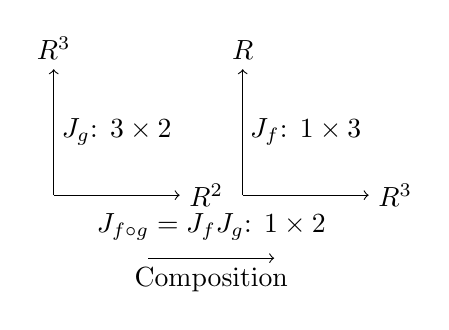
\begin{tikzpicture}[scale=0.8]
\draw[->] (0,0) -- (2,0) node[right] {$\mathbb{R}^2$};
\draw[->] (0,0) -- (0,2) node[above] {$\mathbb{R}^3$};
\node at (1,1) {$J_g$: $3\times 2$};
\draw[->] (3,0) -- (5,0) node[right] {$\mathbb{R}^3$};
\draw[->] (3,0) -- (3,2) node[above] {$\mathbb{R}$};
\node at (4,1) {$J_f$: $1\times 3$};
\draw[->] (1.5,-1) -- (3.5,-1) node[midway,below] {Composition};
\node at (2.5,-0.5) {$J_{f\circ g} = J_f J_g$: $1\times 2$};
\end{tikzpicture}
\]
\end{notechapter}
